\documentclass[english]{article}
\usepackage[T1]{fontenc}
\usepackage[utf8]{luainputenc}
\usepackage{graphicx}
\usepackage{babel}
\title{\textbf{Data acquisition system for the Glass RPC Semi Digital HCAL}}
\author{Guillaume Baulieu\\
		Christophe Combaret\\
		Laurent Mirabito \\
		}
\date{}
\begin{document}

\maketitle
\section{The SDHCAL data acquisition software}
The data acquisition software is splited in three parts: the low
level hardware access that hides  effective hardware implementations,
the configuration data base software handling devices description
and Slow Control parameters and finally the data collection and monitoring. All
packages are written in C++ with interactive scripting in python.
Low level and database C++ libraries are all parsed to python object
with the Swig tool. It allows an interactive instantiation and debug
of single code pieces.


\subsection{The low level hardware access}


\subsubsection{USB readout}

DIF and SDCC FPGA are interfaced with the same USB chip. As mentioned before this is  an
FTDI chip. The DIF is thus uniquely identified by its FTDI device identifier (id) stored in an EEPROM and access to
a specific device id is done using either the proprietary library
FTD2XX or the free version library libFTDI. A device driver library was developped to implement a set of low level access (read and write of registers) of the two boards. 


%A base class called  UsbDeviceDriver (or FtdiDeviceDriver if ftdi library is used) implements
%a set of low level access: bytes read or write , DIF  and SDCC registers
%access and finally predefined commands.


\subsubsection{DIF and SDCC readout}

An upper layer software is dedicated to DIF configuration and
DIF readout. The class DIFDataHandler aggregates a pointer to
a UsbDeviceDriver and to a configuration buffer handling the DIF slow control parameters. Specific methods are used to implement the DIF configuration,
the ASIC configurations and a single event readout to an internal
buffer. Similarly, an SDCCDataHandler implements commands associated to the SDCC.


\subsubsection{DIF Manager}
\label{sec:DIFManager}

Eventually one DIF manager class per PC is responsible of the data
taking of the DIF through the USB connected to it. It handles the DIF and ASIC
configuration parameters via an interface called  DIFManager. This scans and
detects all connected DIF, instantiates one DIFDataHandler class per detected
device and distributes configuration parameters. %and trigger their hardware download. 
When data taking starts, it starts a polling thread continuously
reading events on all connected DIFs. Events can be directly dumped
to disk in LCIO format or transfer to the central data acquisition.
Figure~\ref{software_archi} summarizes the whole architecture.

\begin{figure}
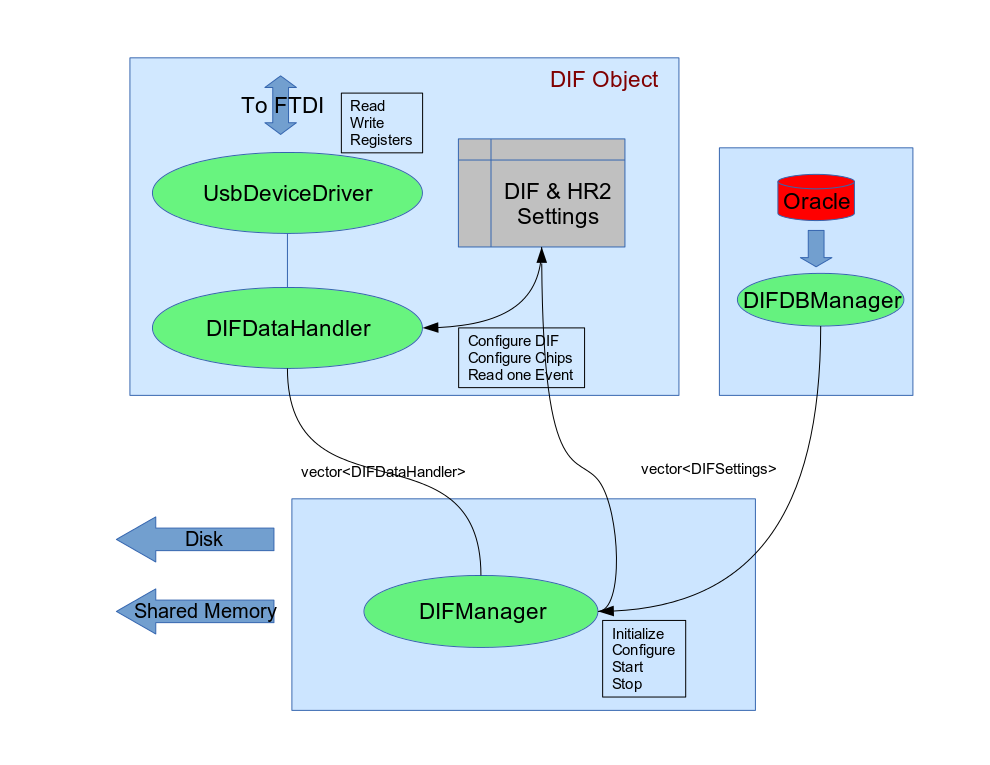
\includegraphics[width=0.9\textwidth]{./LowLevelHardware.png}

\caption{Low level software architecture}
\label{software_archi}

\end{figure}


\subsection{The configuration database}

The configuration database gives the possibility to store and retrieve
all parameters needed by the DAQ system. The database itself is hosted
on an Oracle server at CC IN2P3 (Villeurbanne, France). To interface
this SQL database with the DAQ software and to allow users to insert
and query data without knowledge of SQL, a C++ library has been written.
Part of the DAQ system being written in Python, we used Swig to generate
a Python version of the C++ library. The system has been designed
to easily allow the addition or modification of existing object parameters.
It is built on 2 levels: the database itself and the C++ library.


\subsubsection{Database model}

The database model is conceived to deal with  extendable number of ASIC. It can also handle different kinds of ASIC using different  settings of parameters to take into account addition of other sub-detectors. 
%As an example, we can have different types of ASIC (HardRoc, MicroRoc,...) which need different parameters.
 In this model, each ASIC has a unique entry in the ASIC table, containing its type. The actual configuration parameters
are contained in 2 tables : the first is  ASIC\_CONFIG for the parameters common
to all ASIC types and the second   <ASIC\_TYPE>\_CONFIG for the parameters specific
to a given type. For instance the configuration parameters for a HARDROC
ASIC will be stored in the ASIC\_CONFIG table for the common part
and in the HR2\_CONFIG table for the HARDROC specific parameters\footnote{Here label HR2 is to indicate that we are using the version 2 of the HARDROC ASIC.}.  As a
consequence, supporting a new type of ASIC requires only to create
a new table containing the specific configuration parameters. When
downloading the parameters, the system will automatically choose the
accurate tables associated to the type of the concerned ASIC. 
%Figure~\ref{DataBaseModel} gives an example of 
%\begin{figure}
%\centerline{\[width=0.9\textwidth]{figures/asic_modele2.png}}
%\label{DataBaseModel}
%\caption{Database model: ASIC example}
%\end{figure}



\subsubsection{C++ Library}

All access to the database are done through the C++ library. There
are no mention of the actual configuration parameters in the library
: all names of parameters are retrieved from the database itself at
runtime. The methods used to set or to get parameters value in the
application (API) use the parameters name as an argument (ex : setInt(\textquotedbl{}B0\textquotedbl{},5)
and getInt(\textquotedbl{}B0\textquotedbl{}) ) to respectively set and
retrieve the integer value of the B0 parameter). As a consequence,
there is no need to modify the C++ library when modifying parameters
or adding new types of objects. This will be done dynamically from the
database itself. Each stored configuration is associated with a version
number having the form "MajorID.MinorID". A configuration with version
number 1.0 will contain all the parameters for all the DAQ objects,
whereas a configuration with version number 1.1 will only contain
the modifications from version 1.0. This allows a reduction in the
amount of data to transfer and to store.


\subsubsection{Tools}

The C++ library gives a high level access to the database, providing
the possibility to manipulate the concepts of ASIC, DIF or Configuration
without any SQL knowledge. It allows to create/modify/upload or download
a complete setup defined as follows:

\begin{enumerate}
\item  Setup : a set of \textquotedbl{}states\textquotedbl{} (one per sub-detector)
\item State : a coherent set of \textquotedbl{}configurations\textquotedbl{}
\item Configuration : a list of basic objects 
\item Basic object : a unique object
with all its parameters (ASIC, DIF, DCC, \ldots{}) . 
\end{enumerate}
Figure~\ref{DBSetupStructure}  illustrates the structure of such a setup.
\begin{figure}
\centerline{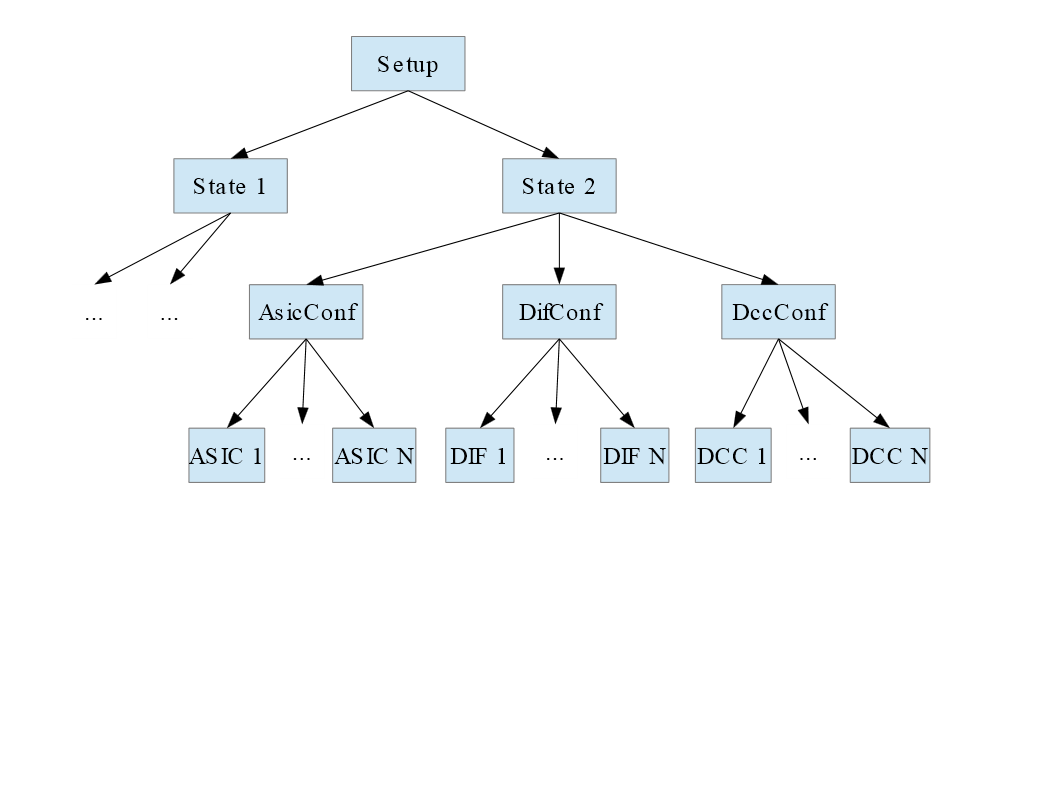
\includegraphics[width=0.9\textwidth]{./setup_structure.png}}
\caption{}
\label{DBSetupStructure}
\end{figure}

In the case of the SDHCAL prototype with 50 active layers, a typical setup contains a single state with 150 DIF,
each having 48 ASICs connected. This corresponds to roughly 550 000
parameters. The download of such a setup takes around 5-7 seconds.
In addition, the library allows to store information about a run
(time, date, type, XDaq configuration, setup used, ...). Using Swig,
a Python version of the C++ library is provided. It is in fact a collection
of python wrappers to the C++ functions. It gives the possibility
to access the database from Python scripts and allows the usage of
the python interpreter as a command line tool to manage configurations.
Finally, configuration setups can be imported/exported to/from the
database using XML files. These files can be used to run an acquisition
without access to the database which could be useful when access to database is interrupted for some reason.
Figure~\ref{DBSoftWare} summarizes the structure of  database access using the different tools.
\begin{figure}[h]
\centerline{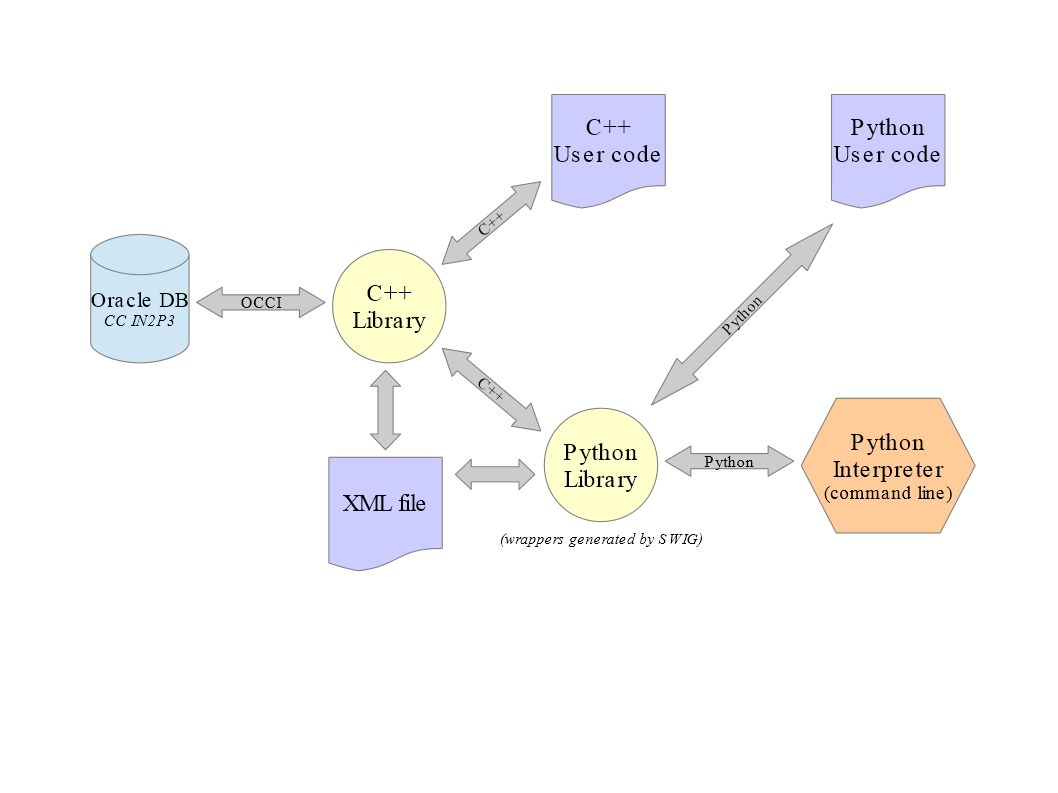
\includegraphics[width=0.9\columnwidth]{./overview.png}}
\caption{Scheme of the database software.}
\label{DBSoftWare}
\end{figure}


\subsubsection{Data acquisition access}

In order to minimize database access during data acquisition, a class called
the DIFDBManager is responsible of the download of all the DIF and ASIC configuration parameters
of a given setup and to cache it for fast access. Data are stored in
indexed maps that provide an instantaneous access to the data needed
by one specific DIF. Each separate DIFManager instantiates one instance
of DIFDBManager and uses it as a configuration cache.


\subsection{The data collection}

\subsubsection{Local data acquisition and coherence}

 In order to  keep the coherence of collected data, DIF  readout outputs are synchronized using the absolute Bunch Crossing ID idedentifier defined in section \ref{sec:DIFfeatures}.
 This is a 48 bits  5 MHz counter that is reset when the first acquisition starts after the DIFs are powered on.  

Data from different DIF may be read out at  different times but will have the same absolute BCID for a given Trigger (or Ramfull) signal.
The logical way to keep synchronicity is to store in a BCID indexed
map the buffers of all read DIF but this requires to manage memory
allocation, access and cleaning. Recent Linux kernels offer the ability
to use shared memory based file, ie, /dev/shm. This special file system
is directly mapped in the system memory and data can be written, listed
and read with extremely fast access. Each DIF data block is written
as a single file named Event\_BCID\_DIFID in /dev/shm and an empty file
/dev/shm/closed/Event\_BCID\_DIFID is created once the event file
is full writen and closed. Standard C functions are used to list events available,
to read, write and delete data. This method allows to separate the
process of reading data from those making data collection, writing,
debugging and monitoring in a single computer without special protocol
or API to be used.


\subsubsection{Global data acquisition with XDAQ}

Whenever several computers are involved in the data taking, a communication
framework is needed. We choose to use the CMS data acquisition XDAQ
framework~\cite{Xdaq}. It provides:
\begin{itemize}
\item A communication with both binary and XML messages.
\item An XML description of the computer and software architecture.
\item A web-server implementation of all data acquisition application.
\item A scalable Event builder.
\end{itemize}
Each PC handling DIFs hold a DIF manager XDAQ application obeying
to a message driven state machine responsible for initialization (
USB scan (section \ref{sec:DIFManager}) and DB download), configuration (DIF and ASIC settings)
and running (DIF readout and /dev/shm storage). A second application
(ShmSupervisor) scans the shared memory and push completed events
to the local event builder application (Readout Unit). The main advantage
of the CMS event builder is the scalability. It is possible to add
any number of collecting application (Builder Unit) that will merge
data from all Readout Units for a given trigger. Those Builder Units
distribute merged events to any analysis and data writing application
(Filter Unit) declared to them. In the SDHCAL case, the computing capability
is handled by the PC's reading the DIF so one Readout Unit, one Builder
Unit and one Filter Unit application are created on each PC as described
on Figure~\ref{SDHCALDAQStructure} and each Filter Unit writes the associated data in a separate stream. 

\begin{figure}
\centerline{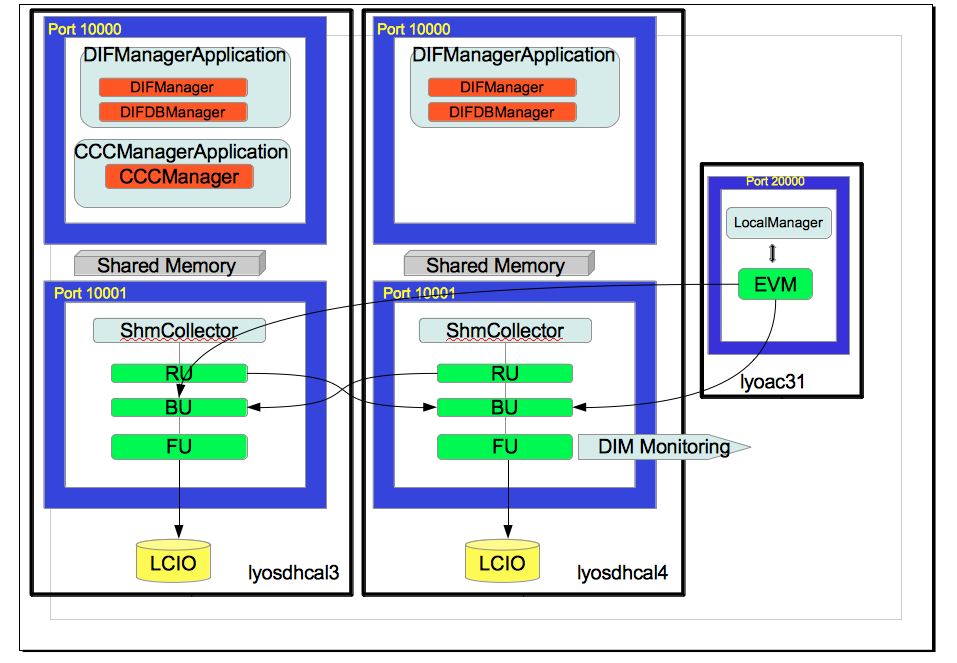
\includegraphics[clip,width=0.85\paperwidth,height=0.4\textheight,keepaspectratio]{./SDHCAL_DAQ_Schema.png}}
\caption{SDHCAL DAQ structure}
\label{SDHCALDAQStructure}
\end{figure}
\subsection{Run Control}
The run control developed in CMS could have been used but its deployment for small beamtest experiment is heavy. Alternatively a set of python script was developed to create XML description of application content of each computer (DIFManager, CCCManager, Database). Then a secondf set of python script used the web capabilities of the XDAQ application and send SOAP or XMLRPC messages to each server to trigger the applications final state machine. 
The global state machine (Initialise, Configure,Enable,Stop,Halt,Destroy) is coded in this python script. Eventually a Qt based graphical user interface is provided, using PyQt \cite{PyQt} framework to bind python methods to graphic widgets. 
\subsection{Online Monitoring}

The online monitoring is a two steps process:
\begin{itemize}
\item A XDAQ application LCIOAnalyzer runs in standalone, waiting for events to be sent by each of the Filter Unit in a sampling mode ($\simeq$ 1\%). Events collected are stored and a separated thread analyzes the events using the ILC analysis program MARLIN \cite{MARLIN} allowing any developers to deploy its own analysis code. The ROOT histograms are booked in memory by a singleton class that keep a map of all histograms booked by any of the analysis modules.

\item The LCIOanalyzer answers to HistoList and HistoGet SOAP commands and returns the list of histograms names and an XML encoding of the histogram requested respectively. Clients, using XMLRPC or SOAP request in python, can 
access the XML answers remotely and using PyROOT \cite{PyROOT} can recovered the request ROOT histogram and display it. Once again a PyQt graphical interface is provided to ease the user access. 
\end{itemize}
This distribution of ROOT histogram is usefull since users are able to manipulate the histogram (zoom, fit...) and not only its image but is limited to a relatively small number of client ( $\simeq$ 10).
\subsection{Performances}

With a 5 Mbit serial bus used to read sequentially the 48 Asics on each ASU, the network is not  

\subsection{Implementation on raspberry pi micro computers}
\subsubsection{Using micro computers}
One critical point in the previous architecture is the number of USB devices that are to be read simultaneously. Moreover since USB bus was originally foreseen as a debug channel the chip only support USB1 (10 Mbit/s) protocol. Reading  150 USB devices on a single PC is then extremely slow and we split it on 4 different PCs with up to 7 bus (42 devices) read in parallel.    


\end{document}
